% !TEX root = SocialVision2014.tex

\Section{Proposed Research}
\label{sec:proposed-research}

Images of human gatherings reveal information about roles and relationships through the visual interactions they depict. The photograph in the bottom-left of Figure~\ref{fig:socialbehavior} suggests the two subjects are close friends because of their apparent proximity, their poses and expressions, and the scene (restaurant/bar) in which they appear. All of these cues are accessible with varying degrees of certainty using existing tools for face detection, pose and expression analysis, and scene recognition; and as described in Sec.~\ref{sec:background}, their utility has already been demonstrated for certain aspects of interaction analysis and social understanding.

Videos contain even richer information about interactions and relationships. In some cases, this can be accessed simply by choosing from the video one keyframe that allows clearer categorization of the interaction, such as the hand-shaking or hugging in Fig.~\ref{fig:socialbehavior}(a). In other cases, much more may be revealed by the spatio-temporal structure of the actors' behaviors. For example, the video before and after the frames in Figs.~\ref{fig:socialbehavior}(b) would reveal attention-response behaviors, turn-taking behaviors, and relative shifts in body position that indicate changes in mutual engagement.

\begin{figure}[b]
\begin{center}
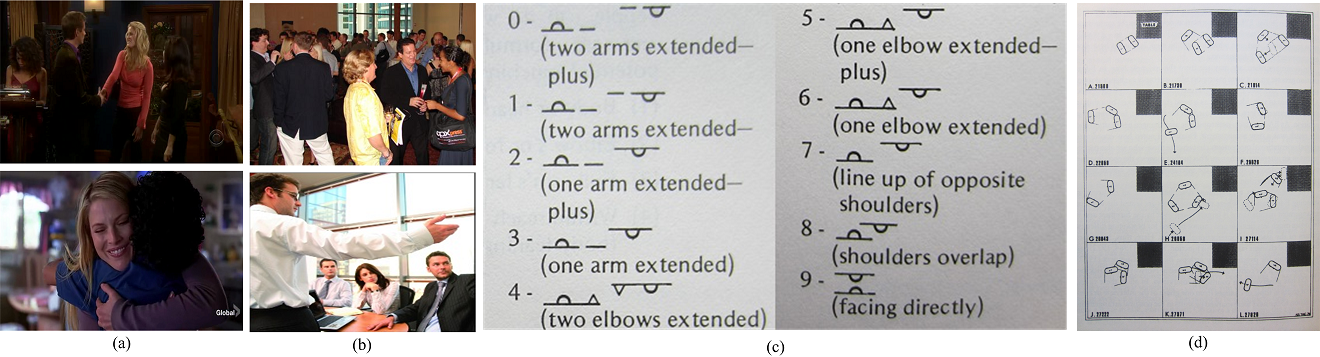
\includegraphics[width=\columnwidth]{socialbehavior_2014}
\end{center}
\vspace{-0.25in} \caption{\captionsize 
Social encounters are ubiquitous (a--b). We will study them and their underlying social relationships by learning and detecting salient environment-specific ``proxemes" as generalizations of those studied in social science (e.g., body configuration spectrum (c) \cite{hall1974} and ``f-formations" (d) \cite{Kendon1990}) in new environments. \label{fig:socialbehavior}\afterfigspace}
\end{figure}





Our goal is to build a computational foundation\comment{for image processing and analysis} that infer the social relationships between every pair of dominant individuals captured in an image/video collection, and this goal must be accomplished by coordinated innovations in semantic image processing and in signal processing on social graph. Semantic image processing aims to localizing the human targets, computing their attributes, recognizing their interactive behaviors (proxemes), and casting relationship estimates on each pair of the targets, after which graph signal processing is required to identify the\comment{ social network of} the unique individuals (nodes), transfer and filter the noisy relationship estimates from target pairs to graph edges, complete the missing edges due to missing co-occurrences, and make joint decisions over all edges to determine the relationship on every edge.

We will employ off-the-shelf tools for semantic image processing tasks to detect and compute the attributes (e.g. gender, age, and occupation, etc.) of the human targets((e.g.,~\cite{LNCS53050340, Gender, Age}), but the focus of our proposed research will be to develop new approaches to detect and recognize instances of \emph{proxemes} --- dictionaries, or categories of elemental, multi-person interaction units that provide a useful intermediate representation between input imagery and the underlying social network. This idea is deeply rooted in the social sciences, where observational studies of human gatherings have repeatedly demonstrated three facts: 1) the nature of visual interactions vary substantially from one setting to the next; 2) within any one setting, customary patterns of visual interaction tend to emerge; and 3) instances of these customary patterns are indicative of the social roles and relationships of the participants. For example, the customary patterns of\comment{head poses, body poses,} poses and gestures\comment{ that emerge} during introductory encounters\comment{ at a cocktail party} are very different from those\comment{ that emerge} in the middle of sustained conversations~\cite{Kendon1990}, and these in turn are very different from the customary patterns for a romantic couple on a park bench~\cite{kendon1975some}, students working around a table~\cite{Scherr2009}, colleagues meeting in a boardroom (Fig.~\ref{fig:socialbehavior}(b)), or students collaborating in comment{ theater-like} lecture hall (Fig.~\ref{fig:prodic}(a)). But in all cases, there are customary behavioral units that emerge, and the enumerated instances of these units--- proxemes---carry valuable information about the social roles and relationships of those participating: Figure~\ref{fig:socialbehavior}(c--d) show two example sets of such proxemes studied by social science, and there are many others.

\comment{
These ideas are well-established but, at present, operationalizing them is a phenomenally onerous task. Social scientists must watch and re-watch many filmed specimens of interaction in a particular setting and do their best to manually identify meaningful, recurring patterns. Figure~\ref{fig:socialbehavior}(c--d) shows two successful examples of this, and there are many others; but this manual approach is fundamentally limited by the availability of human experts, their patience, and their abilities to recognize patterns in large image and video datasets. By creating computational representations and methods that emulate this manual process, we seek to establish a framework for data-driven analysis of visual interactions and relationships that can be applied at transformative scales.This effort is timely because of maturing technologies: As described in Sec.~\ref{sec:background}, a variety of serviceable systems exist, and by integrating them one can extract crude but usable descriptors of individual and relative behaviors in the form of positions, trajectories, histograms-of-flow, bags of interest points, and so on. With these types of features, an image can be abstracted as a noisy collection of positional features, and a video can be abstracted as a noisy collection of space-time features.  The performance of this abstraction will continue to increase as these tools continue to evolve. 
}
%(see Fig.~\ref{fig:intro})

Upon detecting and recognizing a pair of image targets as an instance of a socially-salient proxeme, we will be able to obtain an estimate of relationship types -- a noisy vector-valued observation -- for that pair. We will then develop\comment{ a new suite of} signal processing tools to reconstruct the complete social network among the unique individuals shown in the image/video collection. These tools must address a set of novel challenges to be encountered: First, a unique individual usually repeatedly appears in multiple images or videos and thus gives rise to multiple targets, and these repetitions co-exist with false targets generated by imperfect face/human detectors, unreliable identity similarity scores computed between each pair of image targets, and other spatio-temporal constraints. This requires robust graph coarsening models by which we distill the set of nodes -- the unique dominant individuals -- in the social graph from the massive graph of targets\comment{ connected by the identity similarity scores}. Second, a relationship estimate is not always computable or reliable on every pair of individuals, unless the pair co-occur and perform salient interactions (proxemes) frequently enough.\comment{. Since not everyone interact with everyone else frequently or saliently enough,} Otherwise, relationship estimates must be propagated, by appropriate filters, from observed pairs (edges) with strong proxeme evidences to the edges whose relationship estimate is weak or missing. This requires filtering operating on the multi-dimensional (rather than scalar) relationship signals defined on edges (rather than on nodes) of the social graph, for both ``denoising" and ``prediction". Third, to make a decision about the type relationship between all pairs of nodes, among the estimates of the likelihood over the dictionary of relationships types, one must consider higher-order constraints in relationship specifications, instead of treating each edge independently. This requires multi-way signal detection jointly over all edges while enforcing the higher-order relationship constraints. 

\comment{To meet these challenges, we will extend the state-of-art studies on scalar signals defined on the nodes (0-cell) of a fixed known graph, to the case where graph topology must be inferred before signals on edges (1-cell) can be analyzed and processed. New models and algorithms will be developed, in consolidating ideas of statistical machine learning, but more important in deriving from high-level theoretical abstractions in functional analysis on graph or more generic discrete structure \cite{Grady10}.}

Altogether, we will accomplish the goal in three inter-connected parts: 1) Representing, detecting, and recognizing social proxemes; 2) Robust graph coarsening; and 3) Multi-dimensional signal processing on the graph edges. Simultaneously, we will strive on creating benchmark datasets to evaluate our methods and design challenge problems to engage our colleagues and to enable reproducible research while preserving privacy. The rest of this section details how we will address each of these challenges, measure our progress, and engage our colleagues in this important research agenda.



\subsection{Proxemes and their proximity: The representation space of interactions}
\label{sec:activity}

Among the semantic image processing tools that are necessary for our goal, the focus of our research program deals with learning environment-appropriate proxeme dictionaries, and detecting occurrences of proxemes in novel imagery. At the most basic level, this requires inventing two things: 1) a computational representation of interactions; and 2) a recipe for measuring the similarity (or distance) between two interactions. When co-developing these two things, we have four desiderata. First, they must be discriminative, meaning that the similarity between instances of distinct proxemes should be low while that for instances of the same proxeme should be high. Second, they must be insensitive to distractors, such as changes in occasional occlusions, \comment{participant identities,}temporal extent, and rates of progression within the interaction. \comment{Third, they must be robust and inexpensive, so that we can automatically process large image collections and long videos of large social gatherings.} Third, they must be inexpensive and flexible, meaning that they should be able to maximally exploit varying levels of image information, from low-resolution surveillance video to high-fidelity photographs. fourth and finally, they must accommodate interactions that are hard to describe or encode using explicit grammars, such as required by coupled hidden Markov models~\cite{Brand:CHMM,oliver2000bayesian,mccowan2005automatic}.

\comment{
These desiderata motivate a departure from classical approaches to video, such as coupled hidden Markov models~\cite{Brand:CHMM,oliver2000bayesian,mccowan2005automatic}, that are inspired by speech analysis and represent interactions explicitly as structured per-agent event sequences that are interconnected in time. These approaches can provide very robust detection and recognition of certain types of interactions, but before they can be applied one must optimize for each interaction category the connectivity of atomic events within and between the threads as well as their parameters. This is a daunting task that requires hundreds of cleanly-labeled training samples for each category, and it is not clear how it could be adapted to discover/cluster categories when only few or weak annotations are available.
}
To meet these desiderata, we will develop a new class of interaction representations that are better suited to large-scale, data-driven analysis with less supervision. For videos, our simplest representation is based on ensembles of two types of time-varying descriptors: 1) per-agent descriptors that encode the appearance and/or motion of each agent; and 2) relative pairwise descriptors that encode the appearance and/or motion of each agent relative to another. An interaction spanning $T$ time units (frames or handfuls of frames) and containing $M$ (possibly noisy and fragmented) space-time tracks of agents is represented by the ensemble of $M\cdot T$ per-agent descriptors $\mathbf{f}_{m,t}$ and $M\cdot (M-1)\cdot T$ descriptors $\mathbf{g}_{m,m',t}$ for each agent-pair: ${\cal E}=\{\mathbf{f}_{m,t},\mathbf{g}_{m,m',t} \mid t \in \{1\ldots T\}, m,m' \in \{1\ldots M\} \}$. For images, we use the same representation with $T=1$. Computing the similarity between any two interactions amounts to comparing two ensembles, and detecting new instances of a proxeme amounts to searching through space and/or time for ensembles that are similar to exemplars of that proxeme.

This approach has the advantage of avoiding the explicit description of interaction structure, which is important when an interaction cannot easily be broken down according to any pre-defined grammar, or when one lacks the vocabulary (or aligned and labeled training data) to precisely describe the coupled sequences of per-agent events. It is flexible because the dimension and form of the descriptors $\mathbf{f}$ and $\mathbf{g}$ can be whatever is appropriate for the setting in question, from centroid position and velocity computed from low-resolution surveillance video to more sophisticated descriptors based on space-time interest points, silhouettes, histograms of flow, body pose, expressions, gestures, or higher-level individual action categories. Finally, as we will describe in the remainder of this section, it can be readily combined with matching techniques for comparisons that are insensitive to the distractors described above, allowing us to operationalize the notion of \emph{proxemes} as simple categories of our descriptor-ensembles.








%\comment{In the third part, one should not expect simple one-to-one mappings between proxemes and relationships. Rather, it is the structural distribution of proxemes that matters, in the same way that texton distributions carry information about texture~\cite{leung2001representing} and structured distributions of SIFT descriptors carry information about object and scene categories~\cite{grauman2005pyramid,lazebnik2006beyond}.}



%To the end of our comprehensive framework to sense a social network from visual information, our research agenda on social visual analytics spans two specific major aspects: 1) Detection and recognition of social interaction categories; 2) Social network estimation from multiple visual sources. To facilitate our research activity, we have built up a hardware and software infrastructure as a prototype system and achieved promising preliminary results.

%\begin{figure}[t!]
%\begin{center}
%\includegraphics[width=\columnwidth]{image_feature}
%\end{center}
%\vspace{-0.25in} \caption{\captionsize 
%Socially-informative visual cues from still images: (a-1) Original picture with detected faces; (a-2) relative positions of the detections; (a-3) Facial expressions; (a-4) Relative gazes; (a-5) Relative poses; (a-6) scene recognition. \label{fig:prob1}\afterfigspace}
%\end{figure}

%Images and videos of people reveal information about their interactions, roles, and relationships through a variety cues. The still image in the top-left of Fig.~\ref{fig:intro} suggests the two individuals are friends instead of colleagues because of their proximity, their poses and expressions, and the scene category (restaurant/bar) in which they appear. All of these cues are accessible with varying degrees of certainty using existing tools for face detection, pose and expression estimation, and scene recognition; and their utility for social analysis has already been demonstrated by recent efforts to recover information about age and gender~ \cite{Gallagher}, relationship categories (e.g., father-daughter vs. siblings)~\cite{Wang2010} and event categories (e.g., beach party vs.~country bar)~\cite{Murillo2012}.

%Images and videos of human gatherings reveal information about roles and relationships through the visual interactions they depict. The photograph in the top-left of Fig.~\ref{fig:intro} suggests the two subjects are close friends because of their apparent proximity, their poses and expressions, and the scene (restaurant/bar) in which they appear. All of these cues are accessible with varying degrees of certainty using existing tools for face detection, pose and expression analysis, and scene recognition; and as described in Sec.~\ref{sec:recent-influences}, their utility has already been demonstrated for certain aspects of interaction analysis and social understanding.

%Videos contain even richer information about interactions and relationships. In some cases, this can be accessed simply by choosing from the video one keyframe that allows clearer categorization of the interaction, such as the hand-shaking or hugging in Fig.~\ref{fig:socialbehavior}(a). In other cases, much more may be revealed by the spatio-temporal structure of the actors' behaviors. For example, the video before and after the frames in Figs.~\ref{fig:socialbehavior}(b) would reveal attention-response behaviors, turn-taking behaviors, and relative shifts in body position that indicate changes in mutual engagement.

%\begin{figure}[b]
%\begin{center}
%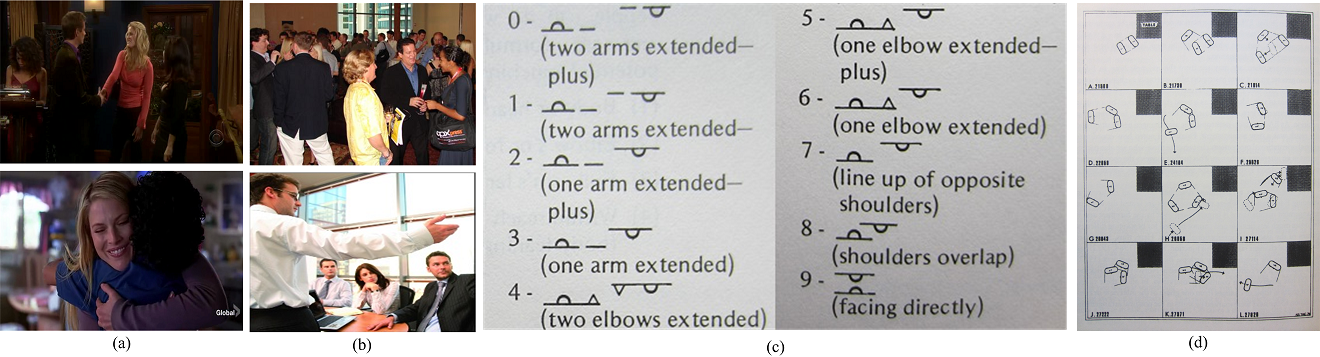
\includegraphics[width=\columnwidth]{socialbehavior_2014}
%\end{center}
%\vspace{-0.25in} \caption{\captionsize 
%Social encounters are ubiquitous (a--b). We will study them and their underlying social relationships by learning and detecting salient environment-specific ``proxemes" as generalizations of those studied in social science (e.g., body %configuration spectrum (c) \cite{hall1974} and ``f-formations" (d) \cite{Kendon1990}) in new environments. 
%(a): Socially non-informative co-occurrence of articulations\cite{UTdata}; (b): Socially non-informative collective crowd activities\cite{Choi:context,Choi:recogtrack,WangMG09}; (c)(d): Socially informative salient interactions; (e) Socially meaningful three-way activity categories defined as `f-formations' by sociology\cite{Kendon1990}.
%\label{fig:socialbehavior}\afterfigspace}
%\end{figure}


%Our goal is to build a computational foundation for social visual analysis by creating tools for extracting as much information as possible about interactions and relationships between people. Our methods will apply to both images, for which social analysis is somewhat established, and videos, for which social analysis is in its infancy; and they will incorporate social interaction categories as a useful intermediate representation between input imagery and the underlying social network. For example, if two individuals are detected as frequently participating in a collegial one-on-one conversation around the water cooler at their workplace, their relationship is likely to be friendly in addition to professional. Similarly, if we observe attention-response instead of turn-taking in a meeting or conversation (Figs.~\ref{fig:socialbehavior}(c--d)) we can recover more detailed information about the interactions and relationships between friends and colleagues.

%Our goal is to build a computational foundation for social visual analysis.  Our approach is based on the idea that dictionaries of \emph{proxemes}---or categories of elemental, multi-person interaction units---provide a useful intermediate representation between input imagery and the underlying social network. This idea is deeply rooted in the social sciences, where observational studies of human gatherings have repeatedly demonstrated three facts: 1) the nature of visual interactions vary substantially from one setting to the next; 2) within any one setting, customary patterns of visual interaction tend to emerge; and 3) instances of these customary patterns are indicative of the social roles and relationships of the participants. For example, the customary patterns of head poses, body poses, and gestures that emerge during introductory encounters at a cocktail party are very different from those that emerge in the middle of sustained conversations~\cite{Kendon1990}, and these in turn are very different from the customary patterns for a romantic couple on a park bench~\cite{kendon1975some}, students working around a table~\cite{Scherr2009}, colleagues meeting in a boardroom (Fig.~\ref{fig:socialbehavior}(b)), or students collaborating in a theater-like lecture hall (Fig.~\ref{fig:prodic}(a)). But in all cases, there are customary behavioral units that emerge, and the enumerated instances these units---or proxemes as we call them---carry valuable information about the social roles and relationships of those participating.

%These ideas are well-established but, at present, operationalizing them is a phenomenally onerous task. Social scientists must watch and re-watch many filmed specimens of interaction in a particular setting and do their best to manually identify meaningful, recurring patterns. Figure~\ref{fig:socialbehavior}(c--d) shows two successful examples of this, and there are many others; but this manual approach is fundamentally limited by the availability of human experts, their patience, and their abilities to recognize patterns in large image and video datasets. By creating computational representations and methods that emulate this manual process, we seek to establish a framework for data-driven analysis of visual interactions and relationships that can be applied at transformative scales.

%Our tools for social visual analysis will apply to both images and videos, and we will develop them in three inter-connected parts: 1) tools for learning and representing dictionaries of environment-specific proxemes; 2) tools for detecting and recognizing instances of these proxemes within larger image and video collections; and 3) tools for using proxeme counts and noisy identities to draw inferences about the underlying social network. \comment{In the third part, one should not expect simple one-to-one mappings between proxemes and relationships. Rather, it is the structural distribution of proxemes that matters, in the same way that texton distributions carry information about texture~\cite{leung2001representing} and structured distributions of SIFT descriptors carry information about object and scene categories~\cite{grauman2005pyramid,lazebnik2006beyond}.}The research we propose is timely because of maturing technologies for detecting and tracking the faces and bodies of people and recognizing their identities. As described in Sec.~\ref{sec:background}, a variety of serviceable systems exist, and by integrating them one can extract crude but usable descriptors of individual and relative behaviors in the form of positions, trajectories, histograms-of-flow, bags of interest points, and so on. With these types of features, an image can be abstracted as a noisy collection of positional features, and a video can be abstracted as a noisy collection of space-time features (see Fig.~\ref{fig:intro}). Our goal is to enable the automatic recovery of useful social based on the features that are available \emph{today}, with the understanding that performance will automatically increase as these tools continue to evolve. Our principal challenge, therefore, is to distill useful information from the substantial and unavoidable uncertainties caused by false detections, broken tracks, noisy features, and erroneous proxeme recognitions. The rest of this section details how we will address these challenges, measure our progress, and engage our colleagues in this important research agenda.

%For example, if two individuals are detected as frequently participating in a collegial one-on-one conversation around the water cooler at their workplace, their relationship is likely to be friendly in addition to professional. Similarly, if we observe attention-response instead of turn-taking in a meeting or conversation, we can recover more detailed information about the relationships between friends and colleagues.

%In order to recover social information from image data, we propose a broad set of tools that enable: 1) representing the space of social interactions in an environment by a discrete set of environment-specific categories; 2) automatically recording over time and space the rates at which different individuals participate in these interaction categories; and 3) using these recordings along with the image data to draw inferences about the underlying social network. Our proposal is inspired by research in sociology~\cite{Kendon1990,Hoyle,Tannen}, economics~\cite{econo_category}, and education~\cite{Scherr2009}, where various social environments  have been  analyzed in terms of a small numbers of interaction categories that are salient and semantically-meaningful (e.g., conversational ``f-formations''~\cite{Kendon1990} in Fig.~\ref{fig:socialbehavior}(e)). It is also motivated by our preliminary results, which suggest that semantically-meaningful interaction categories can reliably be detected and recognized in a real-world (classroom) setting.

%In order to recover social network from image data, we propose a broad set of tools that enable: 1) representing the space of social interactions in an environment by a discrete set of environment-specific proxemes (categories); 2) automatically recording over time and space the occurrences and participants of these proxemes; and 3) using these recordings along with the image data to draw inferences about the underlying social network. 

%Our proposal is inspired not only by research in social sciences\comment{~\cite{hall1974,Kendon1990,Hoyle,Tannen}, economics~\cite{econo_category}, and education~\cite{Scherr2009}} which have analyzed a small number of salient and meaningful proxemes (e.g., conversational body configurations \cite{hall1974}  in Fig.~\ref{fig:socialbehavior} (c) and ``f-formations''~\cite{Kendon1990} in Fig.~\ref{fig:socialbehavior}(d)), 


%but also by our preliminary results suggesting that these proxemes can reliably be detected and recognized in a real-world (classroom) setting. It is also motivated by our experiments showing that new domain-specific proxemes can be discovered in an unsupervised or semi-supervised manner when data is abundant but domain-expert guidance is lacking. (See Section~\ref{sec:activity})



%, and we seek general methods that can exploit inputs of varying precision. High-quality imagery can provide fine-scale information about expression, while low-quality imagery might provide only coarse estimates of head pose. Our goal is to create general tools that operate in all cases and make use of as much information as is available.


%We begin with learning and recognizing interactions and then discuss inferring social network information in Section~\ref{sec:vis2net}. We describe datasets and challenge problems in Section~\ref{sec:sys}. 

%We propose to learn and detect interaction categories (Section \ref{sec:activity}), in complementary to those companion efforts for still images. We then propose to infer social network from images and videos by leveraging all socially-informative visual patterns including occurrences of interactions as an intermediate representation (Section \ref{sec:vis2net}).

%(b-1) Independently recognizing the two faces: The right face is hard to distinguish between two possible people; (b-2) Recognizing faces using social relationship inferred from (a-1) through (a-6): The right face is now more likely to be associated with one person than the other.

%Consider that in recognizing the two faces detected in Fig. \ref{fig:prob1} (a-1) the right face is hard to distinguish between `Susan' and `Helen' (see (b-1)). However, the inferred `friends' relationship suggests that the individual should belong to the left person's list of friends (see (b-2)), which includes only `Helen' but not `Susan'.

%\subsection{Proxemes and their proximity: The representation space of social interactions}
%\label{sec:activity}

%The first part of our research program deals with learning environment-appropriate proxeme dictionaries, and detecting occurrences of proxemes in novel imagery. At the most basic level, this requires inventing two things: 1) a computational representation of interactions; and 2) a recipe for measuring the similarity (or distance) between two interactions. When co-developing these two things, we have four desiderata. First, they must be discriminative, meaning that the similarity between instances of distinct proxemes should be low while that for instances of the same proxeme should be high. Second, they must be insensitive to distractors, such as changes in viewpoint, participant identities, temporal extent, and rates of progression within the interaction. Third, they must be robust and inexpensive, so that we can automatically process large image collections and long videos of large social gatherings. Fourth and finally, they must be flexible, meaning that they should be able to maximally exploit varying levels of image information,  from low-resolution surveillance video to high-fidelity camera networks.

%These desiderata motivate a departure from classical approaches to video, such as coupled hidden Markov models~\cite{Brand:CHMM,oliver2000bayesian,mccowan2005automatic}, that are inspired by speech analysis and represent interactions explicitly as structured per-agent event sequences that are interconnected in time. These approaches can provide very robust detection and recognition of certain types of interactions, but before they can be applied one must optimize for each interaction category the connectivity of atomic events within and between the threads as well as their parameters. This is a daunting task that requires hundreds of cleanly-labeled training samples for each category, and it is not clear how it could be adapted to discover/cluster categories when only few or weak annotations are available.

%that as an explicit \emph{multi-thread event}~\cite{Hongeng:act} comprised of two or more single-thread events (i.e., two or more temporal sequences of per-person atomic actions) that are

%We propose to develop a new class of representations for social interactions that are better-suited to data-driven analysis, including use of techniques like domain adaptation, active learning, semi-supervised learning, and unsupervised learning, which can help reduce the number of training samples to enable widespread use. Our representations are based on ensembles of two types of time-varying descriptors: 1) per-agent descriptors that encode the appearance and/or motion of each agent; and 2) relative pairwise descriptors that encode the appearance and/or motion of each agent relative to another. In the simplest case, an instance of an interaction spanning $T$ time units (frames) and containing $M$ (possibly noisy and fragmented) space-time tracks of agents---these could be centroid locations, bounding boxes, silhouettes, etc.---is simply represented by the ensemble $\{\mathbf{f}_{m,t},\mathbf{g}_{m,m',t}\}$ of $M\times T$ per-agent descriptors $\mathbf{f}_{m,t}$ and $M\times (M-1)\times T$ per-pair descriptors $\mathbf{g}_{m,m',t}$. Computing the similarity between any two interactions amounts to comparing two ensembles, and detecting an interaction category in a long video of a larger social gather amounts to searching through space and time for ensembles that are similar to one or more exemplars in that category. 

%We will develop a new class of interaction representations that are better suited to large-scale, data-driven analysis with less supervision. For videos, our simplest representation is based on ensembles of two types of time-varying descriptors: 1) per-agent descriptors that encode the appearance and/or motion of each agent; and 2) relative pairwise descriptors that encode the appearance and/or motion of each agent relative to another. An interaction spanning $T$ time units (frames or handfuls of frames) and containing $M$ (possibly noisy and fragmented) space-time tracks of agents is represented by the ensemble of $M\cdot T$ per-agent descriptors $\mathbf{f}_{m,t}$ and $M\cdot (M-1)\cdot T$ descriptors $\mathbf{g}_{m,m',t}$ for each agent-pair: ${\cal E}=\{\mathbf{f}_{m,t},\mathbf{g}_{m,m',t} \mid t \in \{1\ldots T\}, m,m' \in \{1\ldots M\} \}$. For images, we use the same representation with $T=1$. Computing the similarity between any two interactions amounts to comparing two ensembles, and detecting new instances of a proxeme amounts to searching through space and/or time for ensembles that are similar to exemplars of that proxeme.

%Our ensemble-based approach has the advantage of avoiding the explicit semantic description of social interactions, which is important when an interaction category cannot easily be broken down according to any pre-defined grammar, or when one lacks the vocabulary to precisely describe the coupled sequences of atomic events that comprise it. It is flexible because the dimension and form of the descriptors $\mathbf{f}$ and $\mathbf{g}$ can be whatever is appropriate for the setting in question, from centroid position and velocity computed from low-resolution surveillance video to more sophisticated descriptors based on space-time interest points, histograms of flow, body pose, expressions, gestures, or higher-level individual action categories. Finally, as we will describe in the remainder of this section, it can be readily combined with matching techniques for comparisons that are insensitive to distractors, allowing applications from learning to detection and recognition.

%Our ensemble-based approach has the advantage of avoiding the explicit semantic description of interactions, which is important when an interaction cannot easily be broken down according to any pre-defined grammar, or when one lacks the vocabulary (or aligned and labeled training data) to precisely describe the coupled sequences of atomic events. It is flexible because the dimension and form of the descriptors $\mathbf{f}$ and $\mathbf{g}$ can be whatever is appropriate for the setting in question, from centroid position and velocity computed from low-resolution surveillance video to more sophisticated descriptors based on space-time interest points, silhouettes, histograms of flow, body pose, expressions, gestures, or higher-level individual action categories. Finally, as we will describe in the remainder of this section, it can be readily combined with matching techniques for comparisons that are insensitive to the distractors described above, allowing us to operationalize the notion of \emph{proxemes} as simple categories of our descriptor-ensembles.

%More precisely,  specifically, assume an input video consisting of $T$ frames. By applying domain-appropriate detection and tracking, assume we obtain $M$ space-time tracks of bounding boxes enclosing $M$ faces or bodies. The $M$ targets are to be compared with an interaction exemplar consisting of $S$ frames and $N$ targets ($N\le M$) that are correctly detected and tracked and all participating in an coherent interaction. Our representation for the input tracks therefore includes $M\times T$ $d_{I}$-dimensional descriptors $\{\mathbf{f}_{m,t}\}_{m=1,2,\cdots,M, t=1,2,\cdots,T}$, where $\mathbf{f}_{m,t}$ encodes the individual activity of the $m$th target at time $t$, and $M\times (M-1)\times T$ $d_{P}$-dimensional pairwise descriptors $\{\mathbf{g}_{m,m',t}\}_{m,m'=1,2,\cdots,M, m\neq m', t=1,2,\cdots,T}$, where $\mathbf{g}_{m,m',t}$ encodes dynamic visual properties of target $m$ exhibited relative to those of target $m'$ at time $t$. Meanwhile, the the interactions of interest are stored as exemplars in a gallery, each exemplar associated with a category label. For each exemplar, we have two similar descriptor collections $\{\mathbf{f}^{D}_{n,s}\}_{n=1,2,\cdots,N, s=1, 2,\cdots, S}$ and $\{\mathbf{g}^{D}_{n,n',s}\}_{n,n'=1,2,\cdots,N, n\neq n', s=1, 2,\cdots, S}$. We denote the descriptor ensemble for the input at time $t$ to be $\mathcal{Q}_{t}\triangleq\{\mathbf{f}_{m,t},\mathbf{g}_{m,m',t}\}$, and that for the exemplar at time $s$ as $\mathcal{D}_{s}\triangleq\{\mathbf{f}^{D}_{n,s},\mathbf{g}^{D}_{n,n',s}\} $. The input is then represented as $\mathcal{Q}\triangleq\{\mathcal{Q}_{t}\}_{1\leq t\leq T}$ and the exemplar $\mathcal{D}\triangleq\{\mathcal{D}_{s}\}_{1\leq s\leq S}$. We show that the can allow efficient measurement of distance in Section \ref{subsec:activity}, and then describe how it serves as a foundation for learning interaction categories in Section \ref{sec:actlearn}.


%We seek to develop new approaches for detecting, localizing, and recognizing these socially informative visual patterns, i.e., interactions, from videos, in complementary to those companion efforts for still images. Through this effort, we foresee a richer set of heterogenous socially informative visual cues from videos in addition to those from images, so as to enable high-level reasoning as to be introduced in Section \ref{sec:vis2net}. 
%We propose a paradigm as to be detailed in Section \ref{subsec:activity}, which is different from the existing work in three aspects. 

%Second, we propose to predict activities under social contexts. In this case, social semantics assist in visual understanding in the way that they serve as contextual information for restricting the more possible categories of activities that may occur between a specific group of individuals. This effort is also complementary to the usage of social contexts for identifying the targets presented in the previous section. Consider a simple illustrative example in which we would like to label a conversational scene in a movie as either a `negotiation� or a 'debate'. It is possible, in this case, that by the analysis of facial expressions, gestures, and poses, we still have difficulty in distinguishing the two. However, by appropriate face recognition in association with other metadata of the movie, probably with the help of social contexts as introduced in the previous section, we may gain solid confidence regarding the social relationship between the speakers as either `cooperative' or 'adverse'. A cooperative relationship are more likely to imply a negotiating activity, and an adverse relationship implies otherwise. A mechanism, similar to and in companion to the CRF formulation but adapted to video analysis, will be particularly useful.

%
%In our following research, we aim to enrich the descriptions of the social behaviors in the current prototype system, explore more accurate and robust comparison and retrieval mechanisms, and in particular, design novel modules for integrating social contextual annotations to allow our framework to be fully `socially-aware'.


%%%%%%%%%%%%%%%%%%%%%%%%%%%%%%%%%%%%%%%%%%%%%%%%%%%%%%%%%%%%%%%%%%%%%%%%%%%%%%%%%%%%%%%%%%%%%%%%%%%%%%%%%

%\subsection{Joint Recognition of Multiple Targets with Social Contexts}
%\label{sec:recognition}
%
%The automatic recognition of targets in image and videos is an central task of computer vision. Recognition of objets is not only essential to any system that seeks to manage visual media based on content, but also necessary for automatically annotating images/videos (`auto-tagging') and indexing them. Recognition of faces is even integral to successfully interpreting images/videos of humans and consequently mining the social semantics in these imagery.
%
%Automatic recognition, since its initial stage until most recently, treats the targets as well as the outputted categories to be independent rom one to the other, which is essentially not the case. In order for automatic recognition to truly succeed, we must exploit the syntactic relationships between targets and between categories and use other contextual information. We in this section propose a scalable computational framework for socially-aware recognition systems that exploit contextual information from online social networks. These online communities provide two significant types of information which, to date, have only been scarcely exploited: 1) significant textual metadata, and 2) social network structure as context. The proposed activity seeks computational foundations for exploiting both.
%
%A typical example of socially-aware face recognition is as follows. A user uploads a small, hundred-image `album' (say)  and we seek to automatically recognize the identities of detected faces in the images. To achieve this goal, we represent the detected faces as nodes in a densely connected, undirected graph. With this representation, recognition consists of estimating a joint labeling of the nodes, which can be formulated as the optimization of an energy-based model. What is unique to our approach is that we seek energy models that combine image information (e.g., classifier output) with contextual information drawn from the user's online social network. Another example is scene recognition, where we seek to jointly label all images with their scene categories in several related online album containing thousands of scene images. Similar examples are more than the two mentioned examples.
%
%The description of an individual target is generally in multiple `views', where a view refers to a specific type of attribute that describes the target. A detected face, for example, can be described by skin color, texture, shape configurations of facial organs, etc.. The description of the contextual network relationship, meanwhile, is also in multiple views. The context between two faces(humans) in Facebook, for example, can be number of their shared friends, the number of their co-occurrence, and their relative poses in images, and so on. As we have mentioned, the social networks are usually partially observed, meaning that not all these views are `visible', and a practically useful recognition system must accommodate the un-observed views for the nodes or the links. Formally,  we can represent  the densely connected, undirected graph as $G$ describing the community of $K$ individuals, where $G\triangleq\{N^{(v_1)},A^{(v_2)},P^{(v_1)}, Q^{(v_2)}\}, v_1=1,2,\cdots,V_1,\hspace{5pt} v_2=1,2,\cdots,V_2$,  $N^{(v_1)}$ is a $K\times 1$ vector describing the individuals in the $v_1$th view, $P^{(v_1)}$ is a $K\times 1$ binary vector describing the visibility for that view, $A^{(v_2)}$ is the $K\times K$ affinity matrix describing the relational context for the $v_2$th view, and $Q^{(v_2)}$ is the $K\times K$ visibility matrix for that view. If $P^{(v_1)}(i)=1$, then $N^{(v_1)}(i)$ is the scalar description of the individual $i$ in the $v_1$th view; otherwise if $P^{(v_1)}(i)=0$ then $N^{(v_1)}(i)$ is a missing number indicating the lack of information of this node in this view. Similar notions apply for the matrices $A$ and $Q$.
%
%With this formulation, a natural computational framework for this socially-aware recognition is a conditional random field (CRF) model~\cite{lafferty2001crf, sutton2007icr, he2004mcr} with a node for each item of interest and an edge connecting many pairs of nodes. In this case, the goal is to infer a joint labeling $\vy=\{y_i\}$ of the relevant categories over all nodes $i$ in the graph. We use the notation $y_i\in{\cal L}=\{l_0\ldots l_M\}$ for the discrete label space of the nodes. (In general, these will vary from node to node, but we use a single set of labels here for notational convenience.) An optimal joint labeling is found by maximizing the conditional density
%\begin{equation} \label{eq:crf}
%{\rm Pr}(\vy|G) = \frac{1}{Z(G)}e^{-E(\vy|G)}
%\end{equation}
%where the partition function $Z(G)$ is a data-dependent normalizing constant and the energy $E(\vy|G)$ consists of sums of unary and pairwise potential functions at the nodes and edges:
%\begin{equation}\label{eq:energy}
%E(\vy|G) =  \sum_{i}  \phi_i (y_i|G) + \sum_{(i,j)} \phi_{ij}(y_i, y_j|G).
%\end{equation}
%
%In the CRF framework, the unary potential functions $\phi_i(y_i|G)$ capture information that is local to each node, and the pairwise potentials $\phi_{ij}(y_i, y_j|G)$ represent the compatibilities of possible label pairs across an edge. Therefore, assuming that the unary potentials depend on individual descriptions and pairwise potentials depend on contextual descriptions, (\ref{eq:energy}) can be decomposed as
%\begin{equation}\label{eq:energy_simple}
%E(\vy|G) =  \sum_{i}  \phi_i (y_i|N,P) + \sum_{(i,j)} \phi_{ij}(y_i, y_j|A,Q).
%\end{equation}
%As part of the proposed activity, we will study the application of this model to practical recognition tasks. Our goal is to answer the following three questions: 1) what types of social network context information improve recognition and by how much?; 2) how should multiple-view of information be weighted and how should missing observation be accounted for?; and 3) how can we apply this model at a practical scale? 
%
%\begin{figure}[t!]
%\begin{center}
%\includegraphics[width=3.5in]{ivw_facescores}
%\end{center}
%\vspace{-0.25in} \caption{\captionsize 
%The performance of a commercial face recognition system on tagged faces harvested from Facebook~\cite{Stone2008}. Given the query face in the upper left, the system has returned the remaining faces as being most similar. Similarity to the query decreases from left to right and from top to bottom, and the ground-truth matches are highlighted with green squares. Due to the variability of this `real-world' dataset, the correct matches are not highly ranked.\label{fig:face-results}\afterfigspace}
%\end{figure}
%
%
%
%\SubSubSection{Preliminary Study}\label{sec:prelim-face-results}
%Evidence for the utility of social network context is provided under simplified assumptions by the work of PI Zickler~\cite{Stone2008,Stone2010}, the former of which received the Best Paper Award at the First IEEE Workshop on Internet Vision. This work reported the results of a preliminary study on the ability of social network context to improve face-based identity recognition using a subset of 2641 labeled faces from Facebook. In this study, we restricted our attention to images with two faces (two-node graphs) so that CRF training and inference could be achieved without approximation. The label space ${\cal L}=\{l_0,\ldots,l_M\}$  consists of a set of possible identities, and we considered a simple set of individual node descriptions and contextual relationship descriptions. Specifically, we assumed that all descriptions in all views are observed and error-free, in which case the potentials in (\ref{eq:energy_simple}) are further expanded as a linear combination of view-specific univariate and bivariate \emph{feature functions} independent of observability variables $P,Q$:
%\begin{eqnarray}
%\phi_i(y_i|N,P) &=& \sum_{v_1} \alpha_{v_1}(N^{(v_1)}) f_{v_1}(y_i, N^{(v_1)})\\
%\phi_{ij}(y_i, y_j|A,Q) &=& \sum_{v_2} \beta_{v_2}(A^{(v_2)}) g_{v_2}(y_i, y_j, A^{(v_2)}).
%\end{eqnarray}
%
%
%\begin{figure}[t!]
%\begin{center}
%\includegraphics[width=5in]{rank_graph_small}\\
%{\footnotesize
%\begin{tabular}{ll}
%\hline\hline\multicolumn{2}{l}{\raisebox{-0.1in}{Univariate Functions $f_{v_1}(y_i, N^{(v_1)})$}} \\
%\hline
%\parbox[t]{1.8in}{\raggedright Face score (\textsf{face})} & \parbox[t]{3.5in}{A distribution of likelihoods over ${\cal L}$ returned by a commercial face recognition system (see Fig.~\ref{fig:face-results})} \vspace{0.03in}\\
%\parbox[t]{1.8in}{\raggedright Photo history (\textsf{hist})} & \parbox[t]{3.5in}{Number of times each individual $l_m$ has been tagged in previous photos posted by the photographer} \vspace{0.07in}\\
%\multicolumn{2}{l}{Bivariate Functions $ g_{v_2}(y_i, y_j, A^{(v_2)})$} \\
%\hline
%\parbox[t]{1.8in}{\raggedright Friendship (\textsf{friend})}& \parbox[t]{3.5in}{Binary indicator that is one iff individuals $l_m$ and $l_n$ are `Facebook friends' } \vspace{0.04in}\\
%\parbox[t]{1.8in}{\raggedright Pairwise co-occurrence (\textsf{pair})}& \parbox[t]{3.5in}{Number of times each pair of individuals $(l_m,l_n)$ has been jointly tagged in previous photos posted by the photographer}\\
%\end{tabular}}
%\end{center}
%\captionspace \caption{\captionsize 
%Face recognition performance as a function of rank threshold for a variety of combinations of feature functions (described bottom). At each rank value $R$, the graph displays the proportion of all test samples for which the correct ground-truth identity label appeared in the top $R$ predictions. Social network context improves recognition, and different sources of context information are complimentary\cite{Stone2008}.\label{fig:ivw-curves}\afterfigspace}
%\end{figure}
%
%
%The results are summarized in Figs.~\ref{fig:face-results} and \ref{fig:ivw-curves}. For each combination of feature functions, we determined model parameters ($\alpha$ and $\beta$) by maximizing the conditional log-likelihood of a training set by gradient ascent. Then, for each left-out test photo, exact marginal probabilities were computed for the test photo's face-nodes, and  the outputs were compared against ground truth. Specifically, the marginal probabilities were used to compute a ranked list at each node, and we measured how often the correct identity label appeared in the top $R$ ranks for a sliding value of $R$ (c.f.~\cite{frvt06}).
%
%A number of observations can be drawn from these results. First, even when using the face score (\textsf{face}) alone (see Fig.~\ref{fig:face-results}) social network context plays a vital role. In our data, over 99\% of tagged faces correspond to `friends' of the photographer, and since the identity of the photographer is known (it is included in the input $N$), we can safely reduce the label space ${\cal L}$ from the 15,752 individuals in the global gallery to the hundreds of friends of the input photographer. Without this restriction, the results in Fig.~\ref{fig:face-results} would degrade remarkably. The results in Fig.~\ref{fig:ivw-curves} also demonstrate that social network context substantially improves baseline face recognition, and that different sources of context information are complementary.
%
%
%These preliminary results are encouraging, especially since the network context information that was employed barely scratches the surface of possibilities. Existing work shows that clothing can provide useful information within an album~\cite{anguelov2007cir, zhang2003aah,  song2006cah, sivic2006fpr}, and it is possible that clothing could be used more globally as well, since the long-term clothing trends of certain individuals may be distinguishable from those of others. Recognition of facial attributes~\cite{LNCS53050340}, such as glasses or facial hair, can be used in conjunction with identity scores to improve recognition, and the same is true for gender recognition, which in many online communities is a knowable piece of information. In addition, people associate with each other in homes, schools, outdoors, workplaces, clubs, and so on, and a more explicit representation of these would be beneficial. Certain individuals will appear more often in certain types of scenes, and these `likely' scene types will change depending on who they are with. Temporal and geographic information, when available, may be further predictive of which individual is likely to occur and with whom. 
%
%
%
%In our proposed research, we aim to both qualitatively and quantitatively analyze large collections of images and their embedding network to discover the utility of these multi-view context information, and in particular, explore effective approaches to account for incompletely observed graph, which is the crucial to allow our framework to succeed in realistic network conditions.